\chapter{Implementation}
\label{ch:implementation}

\section{HDL structure}
Implementation starts from the block diagram described in Chapter \ref{ch:design}, moving from that to laying out the HDL skeleton within Scala. Both Chisel bundles (collections of inputs and outputs used to define interfaces) and Chisel modules are Scala classes, so the layout of the code follows a standard Java/Scala package layout \cite{scala_style}. The top-level package is \txt{dev.joeyh.pio} (the author's domain is \txt{joeyh.dev}), containing the following sub-packages and files

\begin{itemize}
    \item \txt{execution} - The execution unit and sub-components
          \begin{itemize}
              \item \txt{ExecUnit} - The top-level execution unit
              \item \txt{Decode} - Instruction decoder
              \item \txt{ProgramCounter} - PC register
              \item \txt{Branch} - JUMP execution unit
              \item \txt{Move} - MOV/SET execution unit
              \item \txt{Wait} - WAIT execution unit
          \end{itemize}
    \item \txt{fifo} - FIFOs and reusable interface definitions
          \begin{itemize}
              \item \txt{Fifo} - The FIFO module and sub-components, used for both RX and TX FIFOs
              \item \txt{ProducerIO} - Bundle definition for FIFO producer
              \item \txt{ConsumerIO} - Bundle definition for FIFO consumer
          \end{itemize}
    \item \txt{shiftreg} - Shift registers
          \begin{itemize}
              \item \txt{ISR} - Input shift register
              \item \txt{OSR} - Output shift register
              \item \txt{ShiftRegIO} - Common shift register interface definitions
          \end{itemize}
    \item \txt{memory} - Shift registers
          \begin{itemize}
              \item \txt{CSR} - Control and status register file
              \item \txt{InstructionMem} - 32x16bit Instruction memory
              \item \txt{ScratchReg} - 32-bit scratch register
          \end{itemize}
    \item \txt{util} - Miscellaneous reusable components and utilities
          \begin{itemize}
              \item \txt{Random} - functions for generating random Chisel \txt{UInt}s, used for testing
              \item \txt{ReadWrite} - reusable read and write port interface definitions
          \end{itemize}
\end{itemize}

Some files contain one (or more) Chisel modules, while others contain bundle definitions that are designed to be reused accross multiple modules. Bundles as types is a great feature of Chisel, as it allows to abstract over them using the connection operators. The module hierarchy of the overall design from this is fairly flat, shown in Figure \ref{fig:hdl_hierarchy}.

\begin{figure}[H]
    \centering
    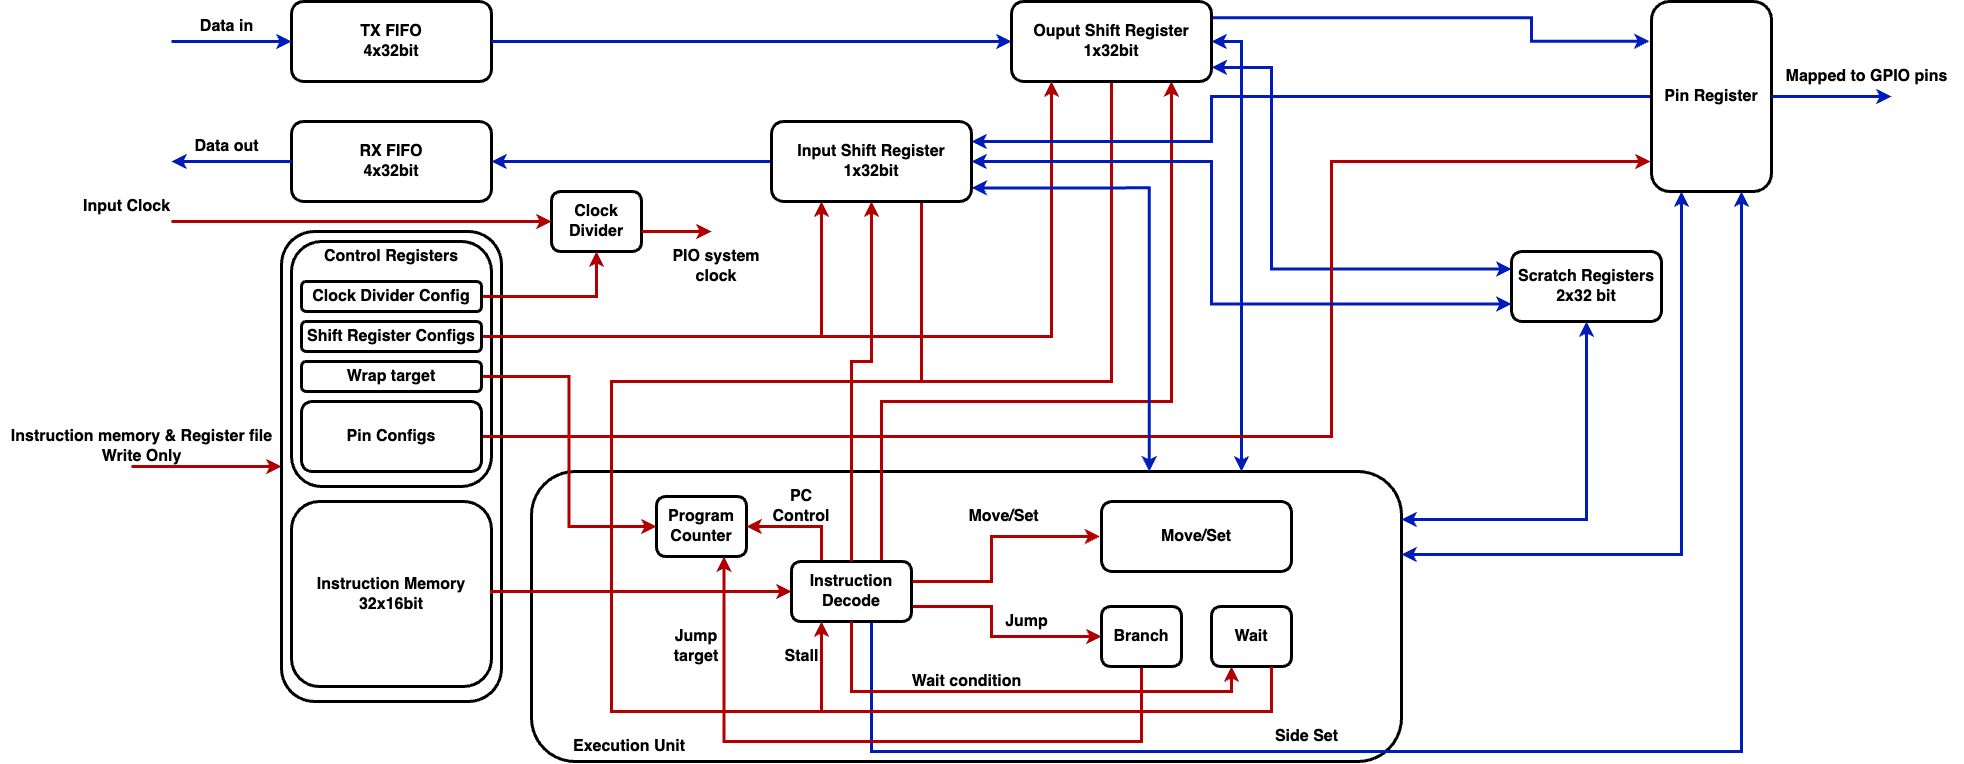
\includegraphics[width=0.9\textwidth]{../img/bd.png}
    \caption{The modular, hierarchical design of the PIO.}
    \label{fig:vivado-bd}
\end{figure}

\section{Execution Unit}

\section{FIFOs}

\section{Shift Registers}

\section{Pin Mapping}

\section{Other Components}

\section{AXI Wrapper}

\section{Chisel Abstractions}